\documentclass[tikz,border=10pt]{standalone}
\usepackage{tikz}
\usepackage{fontawesome5}
\usetikzlibrary{arrows.meta,positioning,fit,backgrounds,calc,shadows,shapes.geometric}

\definecolor{civNavy}{RGB}{15, 34, 64}
\definecolor{civBlue}{RGB}{28, 80, 160}
\definecolor{civTeal}{RGB}{14, 130, 120}
\definecolor{civLightBlue}{RGB}{238, 245, 255}
\definecolor{civBorder}{RGB}{185, 210, 240}
\definecolor{civGold}{RGB}{217, 119, 6}
\definecolor{civGreen}{RGB}{22, 130, 80}
\definecolor{civDark}{RGB}{20, 28, 42}
\definecolor{cInput}{RGB}{240, 246, 255}
\definecolor{cStem}{RGB}{224, 242, 254}
\definecolor{cStage1}{RGB}{209, 250, 229}
\definecolor{cStage2}{RGB}{254, 243, 199}
\definecolor{cStage3}{RGB}{254, 226, 226}
\definecolor{cStage4}{RGB}{236, 254, 255}

\begin{document}
% Complete Layered System Workflow for CiviQ Civic Grievance Platform
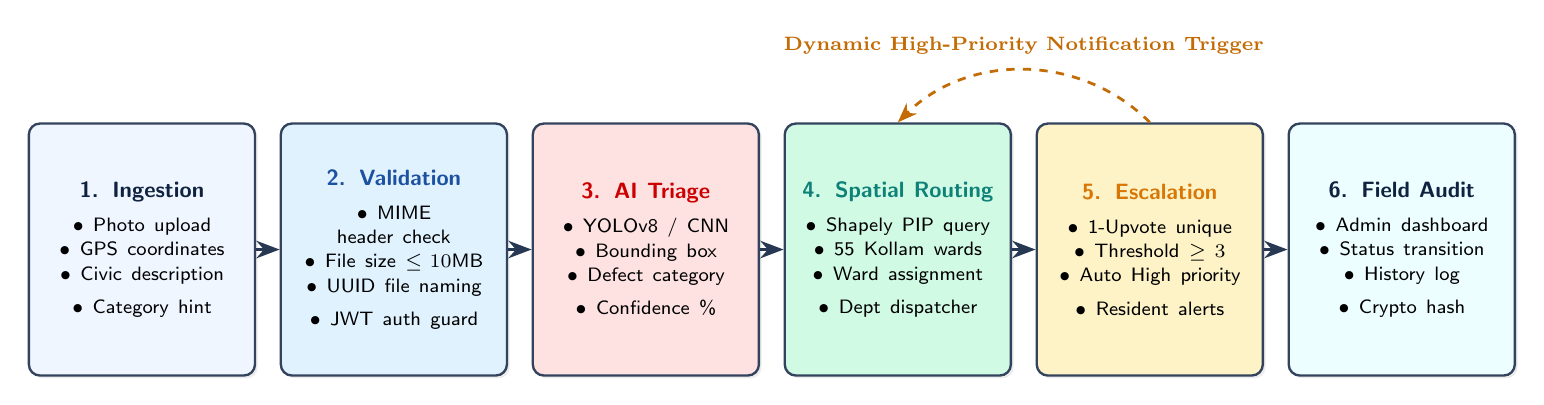
\begin{tikzpicture}[
    x=1cm, y=1cm,
    font=\sffamily,
    stepbox/.style={
        rectangle, draw=civNavy!85, line width=0.85pt, fill=white,
        rounded corners=4pt, inner sep=6pt, align=center,
        minimum height=3.2cm, text width=2.45cm,
        drop shadow={shadow xshift=1pt, shadow yshift=-1pt, opacity=0.15}
    },
    flowarr/.style={
        -{Stealth[scale=1.0]}, line width=1.2pt, draw=civNavy!90
    },
    dashloop/.style={
        -{Stealth[scale=0.95]}, line width=1.0pt, dashed, draw=civGold!90!black
    }
]

    % Step 1: Grievance Ingestion
    \node [stepbox, fill=cInput] (b1) at (0, 0) {
        \textbf{\fontsize{8.5}{10.0}\selectfont\color{civNavy}1. Ingestion}\\[0.35em]
        \fontsize{7.2}{8.8}\selectfont
        $\bullet$ Photo upload\\
        $\bullet$ GPS coordinates\\
        $\bullet$ Civic description\\
        $\bullet$ Category hint
    };

    % Step 2: Validation & Sanitization
    \node [stepbox, fill=cStem] (b2) at (3.2, 0) {
        \textbf{\fontsize{8.5}{10.0}\selectfont\color{civBlue}2. Validation}\\[0.35em]
        \fontsize{7.2}{8.8}\selectfont
        $\bullet$ MIME header check\\
        $\bullet$ File size $\le 10$MB\\
        $\bullet$ UUID file naming\\
        $\bullet$ JWT auth guard
    };

    % Step 3: AI Computer Vision Triage
    \node [stepbox, fill=cStage3] (b3) at (6.4, 0) {
        \textbf{\fontsize{8.5}{10.0}\selectfont\color{red!80!black}3. AI Triage}\\[0.35em]
        \fontsize{7.2}{8.8}\selectfont
        $\bullet$ YOLOv8 / CNN\\
        $\bullet$ Bounding box\\
        $\bullet$ Defect category\\
        $\bullet$ Confidence \%
    };

    % Step 4: Geospatial PIP Routing
    \node [stepbox, fill=cStage1] (b4) at (9.6, 0) {
        \textbf{\fontsize{8.5}{10.0}\selectfont\color{civTeal}4. Spatial Routing}\\[0.35em]
        \fontsize{7.2}{8.8}\selectfont
        $\bullet$ Shapely PIP query\\
        $\bullet$ 55 Kollam wards\\
        $\bullet$ Ward assignment\\
        $\bullet$ Dept dispatcher
    };

    % Step 5: Community Escalation
    \node [stepbox, fill=cStage2] (b5) at (12.8, 0) {
        \textbf{\fontsize{8.5}{10.0}\selectfont\color{civGold}5. Escalation}\\[0.35em]
        \fontsize{7.2}{8.8}\selectfont
        $\bullet$ 1-Upvote unique\\
        $\bullet$ Threshold $\ge 3$\\
        $\bullet$ Auto High priority\\
        $\bullet$ Resident alerts
    };

    % Step 6: Redressal & Audit
    \node [stepbox, fill=cStage4] (b6) at (16.0, 0) {
        \textbf{\fontsize{8.5}{10.0}\selectfont\color{civNavy}6. Field Audit}\\[0.35em]
        \fontsize{7.2}{8.8}\selectfont
        $\bullet$ Admin dashboard\\
        $\bullet$ Status transition\\
        $\bullet$ History log\\
        $\bullet$ Crypto hash
    };

    % Forward Pipeline Arrows
    \draw [flowarr] (b1) -- (b2);
    \draw [flowarr] (b2) -- (b3);
    \draw [flowarr] (b3) -- (b4);
    \draw [flowarr] (b4) -- (b5);
    \draw [flowarr] (b5) -- (b6);

    % Feedback Loop Arrow (Escalation to Redressal)
    \draw [dashloop] (b5.north) to[out=135, in=45] 
        node[above=2pt, font=\fontsize{7.0}{8.5}\selectfont\bfseries, text=civGold!90!black] 
        {Dynamic High-Priority Notification Trigger} (b4.north);

\end{tikzpicture}
\end{document}
